\section{Structural   Mechanics  model\todo{Till}}   Static  structure
mechanics  problems  can be  handled  using  the structural  mechanics
model.  So far,  \akantu\ provides 2D and 3D  Bernouilli beam elements
\cite{REFERENCE}.   Just as  for  the \code{SolidMechanicsModel},  the
model is created  for a given \code{Mesh}.  The  model will create its
own  \code{FEM}   object  to  compute   the  interpolation,  gradient,
integration        and         assembly        operations.         The
\code{StructuralMechanicsModel} constructor is used like

\begin{cpp}
  StructuralMechanicsModel model(mesh, spatial_dimension);
\end{cpp}

where  \code{mesh} is  a  \code{Mesh}  object defining  the
structure for  which the  equations of statics  are to be  solved, and
\code{spatial\_dimension}  is the dimensionality  of the  problem.  If
\code{spatial\_dimension} is  omitted, the problem is  assumed to have
the same  dimensionality as the one  specified by the  mesh. Note that
dynamic computations are not supported to date.


This model contains at least the the following \code{Vectors}:
\begin{description}
\item[boundary]  contains a  \code{boolean} value  for each  degree of
freedom specifying whether that degree  is blocked or not. A Dirichlet
boundary condition can be  prescribed by setting the \textbf{boundary}
value  of a  degree of  freedom  to \code{true}.   A Neumann  boundary
condition  can only  be applied  if the  \textbf{boundary} value  of a
degree  of freedom  is  \code{false}. If  a  degree of  freedom has  a
\textbf{boundary}     value      that     is     \code{false},     the
\textbf{displacement},  \textbf{velocity},  \textbf{acceleration}  and
\textbf{residual} are  computed by the solve  algorithm when relevant,
otherwise  these vectors contain  the imposed  value (zero  by default
after the initialization).
  
\item[displacement    and   rotation]    contains    the   generalized
displacements of all  degrees of freedom. It can  be either a computed
displacement for free degrees of freedom or an imposed displacement in
case of blocked ones ($\vec{u}$ in the following).
  
\item[force  and  moment]  contains  the generalized  external  forces
applied to the nodes ($\vec{f_{\st{ext}}}$ in the following).
  
\item[residual] contains the  difference between external and internal
forces and  moments. On blocked degrees  of freedom, \textbf{residual}
contains  the support  reactions.  ($\vec{r}$  in the  following).  It
should be  mentioned that  at equilibrium \textbf{residual}  should be
zero on free degrees of freedom.
\end{description}

Some examples  to help  to understand  how to use  this model  will be
presented in the next sections.

\subsection{Model setup}
\label{sec:structMechMod:setup}

\subsubsection{Initialization}
Material  properties are  defined using  the \code{StructuralMaterial}
structure described in Table~\ref{tab:structMechMod:strucMaterial}.  
\begin{table}[htb] \centering
  \begin{tabular}{c|c} field  & description \\\hline\hline
    \code{E} & Young's  modulus  \\\hline
    \code{A}  & Cross  section  area  \\\hline
    \code{I} & Second cross sectional  moment of inertia (for 2D elements)
    \\\hline \code{Iy} & \code{I}  around beam $y$--axis (for 3D elements)
    \\\hline \code{Iz} & \code{I}  around beam $z$--axis (for 3D elements)
    \\\hline \code{GJ}  & Polar  moment of inertia  of beam  cross section (for 3D elements)
  \end{tabular}
  \caption{Material properties  for structural elements  as defined by
the structure \code{StructuralMaterial}.}
  \label{tab:structMechMod:strucMaterial}
\end{table}
The structural mechanics model is  initialized in a few steps:
\begin{cpp}
  model.initModel();
  
  StructuralMaterial mat1;
  mat1.E=2.05e11;
  mat1.I=0.00128;
  mat1.A=0.01; // for example

  model.addMaterial(mat1); ASK NICO ABOUT THIS CRAP

  model.initVectors();
  model.initImplicitSolver();
\end{cpp}

The method \code{initModel} computes the shape functions, \code{addMaterial} sets the material parameters to be used, \code{initVectors} initializes all the internal vectors mentioned before and \code{initImplicitSolver} creates the stiffness matrix.

\subsubsection{Setting boundary conditions}

Both Dirichlet and Neumann type boundary conditions are applied to nodes the same exact way as for \code{SolidMechanicsModel}, see Section~\ref{sect:smm:boundary}. Additionally, \code{SolidMechanicsModel} provides the methods \code{computeForcesByStressTensor}, \code{computeForcesByTractionVector} and \code{computeForcesFromFunction} to compute consistent forces from applied constant stresses, constant tractions

\subsection{Static analysis\label{sect:smm:static}}

The \code{SolidMechanicsModel} class can  handle different analysis methods, the
first one being presented is the static case.  In this case, the equation
to solve is,
\begin{equation}\label{eqn:smm:static}
  \mat{K} \vec{u} = \vec{f_{\st{ext}}}~,
\end{equation}
where  $\mat{K}$ is  the  global stiffness  matrix,  $\vec{u}$ the  displacement
vector  and  $\vec{f_{\st{ext}}}$ the  external  forces  vector  applied to  the
system.


To     solve    such     a    problem     the    static     solver     of    the
\code{SolidMechanicsModel}\index{SolidMechanicsModel}  object is used.   First a
model has to be  created and initialized.  To create the model,  a mesh that can
be read from  a file is needed, as  explained in section \ref{sect:common:mesh}.
Once an instance of a \code{SolidMechanicsModel} is obtained, the easiest way to
initialize it is  to use the \code{initFull}\index{SolidMechanicsModel!initFull}
function by  giving a  material file containing  the material parameters,  and a
type of analysis.

\begin{cpp}
  SolidMechanicsModel model(mesh);
  model.initFull("material.dat", _static);
\end{cpp}


\begin{itemize}
\item \code{model.initFull}  initializes all the  needed vectors to zero.   If a
  material file is given it also  parses it and creates the requested materials.
  The last  parameter of this function  is the type  of solver to use.  Here the
  \code{\_static} solver is used.
\end{itemize}


Once the model is created and  initialized the boundary conditions can be set as
explained   in  section   \ref{sect:smm:boundary}.   Boundary   conditions  will
prescribe   the   external   forces    for   the   free   degrees   of   freedom
$\vec{f_{\st{ext}}}$ and displacements for the others.  To completely define the
system  represented  by equation  (\ref{eqn:smm:static}),  the global  stiffness
matrix            $\mat{K}$             must            be            assembled.
\index{SolidMechanicsModel!assembleStiffnessMatrix}

\begin{cpp}
  model.assembleStiffnessMatrix();
\end{cpp}

In fact, to find the  equilibrium, Equation (\ref{eqn:smm:static}) is modified in
order to apply a Newton-Raphson convergence algorithm.

\begin{align}\label{eqn:smm:static-newton-raphson}
  \mat{K}^{i+1} \delta\vec{u}^{i+1} &= \vec{r} \\
  &= \vec{f_{\st{ext}}} - \vec{f_{\st{int}}}\\
  &= \vec{f_{\st{ext}}} - \mat{K}^{i} \vec{u}^{i}\\
  \vec{u}^{i+1} &= \vec{u}^{i} + \delta\vec{u}^{i+1}~,\nonumber
\end{align}
where $\delta\vec{ u}$ is the  increment of displacement  to be added  from one
iteration to the other, and $i$ is the number of the Newton-Raphson iteration.

So  in  a  Newton-Raphson  iteration,  $\mat{K}$ is  updated  according  to  the
displacement computed at  the previous iteration and one  loops until the forces
are balanced, \ie $\vec{r} = 0$.  One can also iterate until the increment of
displacement is zero which also means that the equilibrium is found. This can be
done as follow:
\index{SolidMechanicsModel!updateResidual}
\index{SolidMechanicsModel!solveStatic}

\begin{cpp}
  model.updateResidual();
  model.solveStatic();
\end{cpp}
\begin{itemize}
\item \code{model.updateResidual} assembles the  internal forces and remove them
  from the external forces.
\item        \code{model.solveStatic}         solves        the        equations
  (\ref{eqn:smm:static-newton-raphson}).   The \textbf{increment} vector  of the
  model   will   contain  the   new   increment   of   displacements,  and   the
  \textbf{displacement} vector is also updated to the new displacements.
\end{itemize}

For  an   elastic  problem  the  solution   is  directly  found   at  the  first
iteration. But for a non-elastic case, one  needs to iterate as long as the norm
of the residual is not zero (given a specific tolerance).
\begin{cpp}
  Real norm;
  Real tolerance = 1e-3;
  UInt count = 0;
  model.updateResidual();
  while(!model.testConvergenceResidual(tolerance, norm) && (count < 100)) {
    model.solveStatic();
    model.updateResidual();
  };
\end{cpp}

At   the  end   of  the   analysis  the   final  solution   is  stored   in  the
\textbf{displacement} vector.  A  full example of how to  solve a static problem
is  presented  in   the  code  \code{example/manual/implicit\_static.cc}.   This
example is composed of a 2D plate of steel, blocked with rollers on the left and
bottom sides as shown in  Figure \ref{fig:smm:static}.  The nodes from the right
side of the sample are displaced by $0.01\%$ of the length of the plate.

\begin{figure}[!htb]
  \centering
  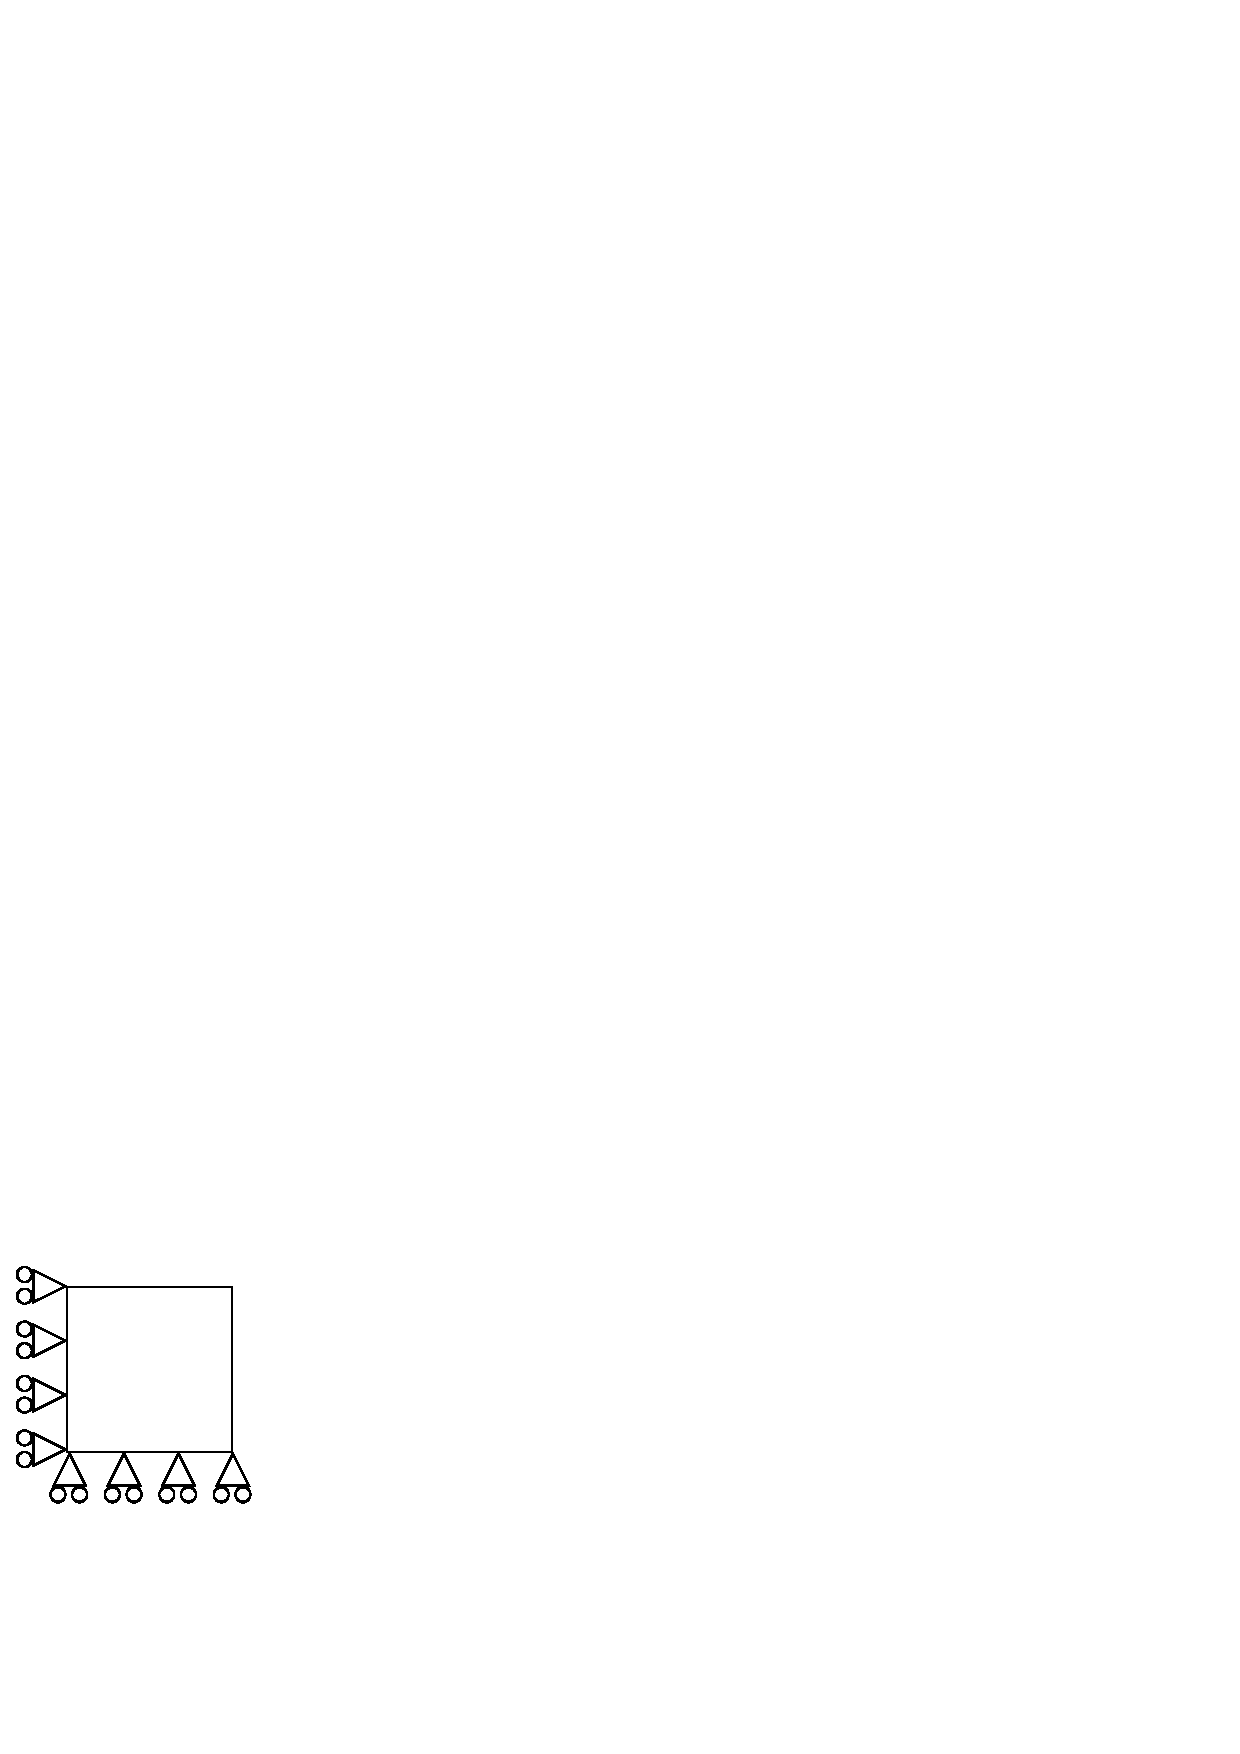
\includegraphics{figures/implicit_static}
  \caption{Numerical setup\label{fig:smm:static}}
\end{figure}

The     results     of    this     analysis     is     depicted    in     Figure
\ref{fig:smm:implicit:static_solution}.

\begin{figure}[!htb]
  \centering
  \includegraphics[width=.6\linewidth]{figures/static_analysis}
  \caption{Solution of the static  analysis. Left: the initial condition, right:
    the solution (deformation magnified 50 times)}
  \label{fig:smm:implicit:static_solution}
\end{figure}



%%% Local Variables: %%% mode: latex %%% TeX-master: "manual" %%% End:


